This discussion is structured into two semi-independent parts: We first summarize the results from the simulation study and reflect on how we can develop on the methods, especially on the numerical optimization side of things. Furthermore, we mention two estimation methods that could be interesting to consider in future research.

Then we put the results from the estimation of the AMOC into perspective, contrasting it with previous findings. Here, we also discuss how one might go about selecting between models from \ref{table:ergodicDiffusions}. In particular, with our models as a starting point, we discuss what type of role the stochastic part in these types of analysis can have. Additionally, we mention a couple of other ideas that can be used on these models in practice. In extension, we reflect on how one can think about these models in general.
\subsection{Simulation Studies}
Our starting point for the discussion is a short look into the results shown in Figures \ref{figure:parameter_precision_dynamic} and \ref{figure:overviewOfEstimatorsStationary}. As we noted it is not given that the behaviour shown in these graphs is representative on all scales. Additionally, the experiment only tweaked the number of samples through the temporal resolution. In a future study, it would be interesting to investigate how longer (or shorter) time series affect the estimators in an otherwise similar experiment. With our simulation schemes, we can achieve this by changing the $t_0$- and $\tau_c$ parameters.

Another natural extension is to look into other evaluation metrics. We mostly considered the ARE and the computation time. One other metric we could have used more is the relative error. Another popular choice is just the difference between the estimate and the true value because it, with proper normalization, can be used to examine the distribution of the estimators more precisely. Although we have not stated them, many of our estimators have asymptotic results, which in principle can be demonstrated in these kinds of studies.\\\\
Other than that, we could consider changing the BFGS algorithm to other algorithms and study what effect tweaking potential hyperparameters for these might have. In continuation, specifying the gradients for the various methods might reduce the number of steps required for convergence at the minimum. Having a closed form of the gradient likely makes evaluating it less computationally heavy than our current implementation as \code{stats::optim} uses finite-difference-based methods, when no gradient is provided. Albeit, in our current development the Ornstein Uhlenbeck is the only process for which we have implementations of both the likelihood and the score. However, to motivate further research, we conducted a small experiment that shows that the optimization can gain significantly from our providing a gradient to it. The result is shown in table \ref{table:smallOUExperiment}. To be able to apply the strategy outside of this case hinges on the Strang-based score being tractable. But if it were, then we could use it in unison with the likelihood in the optimization. We also briefly considered using the martingale estimation equations from the mean-reverting GBM in unison with its Strang-based pseudo-likelihood. This was a bit more troublesome to get to work and the results were not as convincing, so we let that be up to further research.  \\\\
Moving on, there is no doubt that at our current state of implementation, it is not feasible to estimate with a varying $\nu$-parameter in the models. As seen in Figure \ref{figure:error_count_nu_experiment} the optimization process is simply not robust enough to even try estimation on real data. It is probable that the challenges we have experienced stem from the fact that $\nu$ enters into the likelihood in quite a complex manner. Confer Figure \ref{figure:nu_plot}, the $\nu$-parameter shapes the overall evolution of the fixed point. What the plot also reveals is that relatively small changes around $\nu = 1$ result in quite different shapes, making estimation difficult.
 
Without any prior knowledge, the idea of starting optimization at $\nu = 1$ seems like the only fair way to do so. So before we find any reasons to deviate from this we stick with this strategy. However, this can obviously leave the optimizer with a difficult optimization problem; there is a chance we get stuck in local minima or it simply is infeasible if this initial value is too poor given the data. To remedy the first issue, one option we could try is to penalize values of $\nu$ relatively far away from $1$. Due to the form (\ref{eq:lambdaRampDefinition}) straying further away from $\nu = 1$ results in progressively smaller changes in the shape for a change in $\nu$. In Figure \ref{figure:nu_plot} this can be seen by the shape of the fixed points not being as different for $\nu = 2.27$ and $\nu = 4.48$ as for instance $\nu = 1$ to $\nu = 1.65$. Therefore penalizing values much larger than $1$ and relatively close to $0$ might be a good choice to push the optimization away from these parts of the parameter space. In continuation of our discussion about providing gradients to the optimizer, the issue at hand might be another use case of this as lack of robustness might stem from the finite-difference-based methods used by \code{stats::optim} here. \\\\
When the optimization of $\nu$ is more robust another consideration to make is to question when there even is enough information in the time series to estimate $\nu$ reliably. We would have liked to investigate this with a simulation study. Unfortunately due to the aforementioned issues, we can only illustrate this point intuitively here. To do so, we sample from the additive-noise model using the same parameters as in Figure \ref{figure:nu_plot}. The $\sigma$-parameter is set to $0.3$ and we sample with temporal resolution $\Delta t = 1/24$
\begin{figure}[h!]
    \begin{center}
    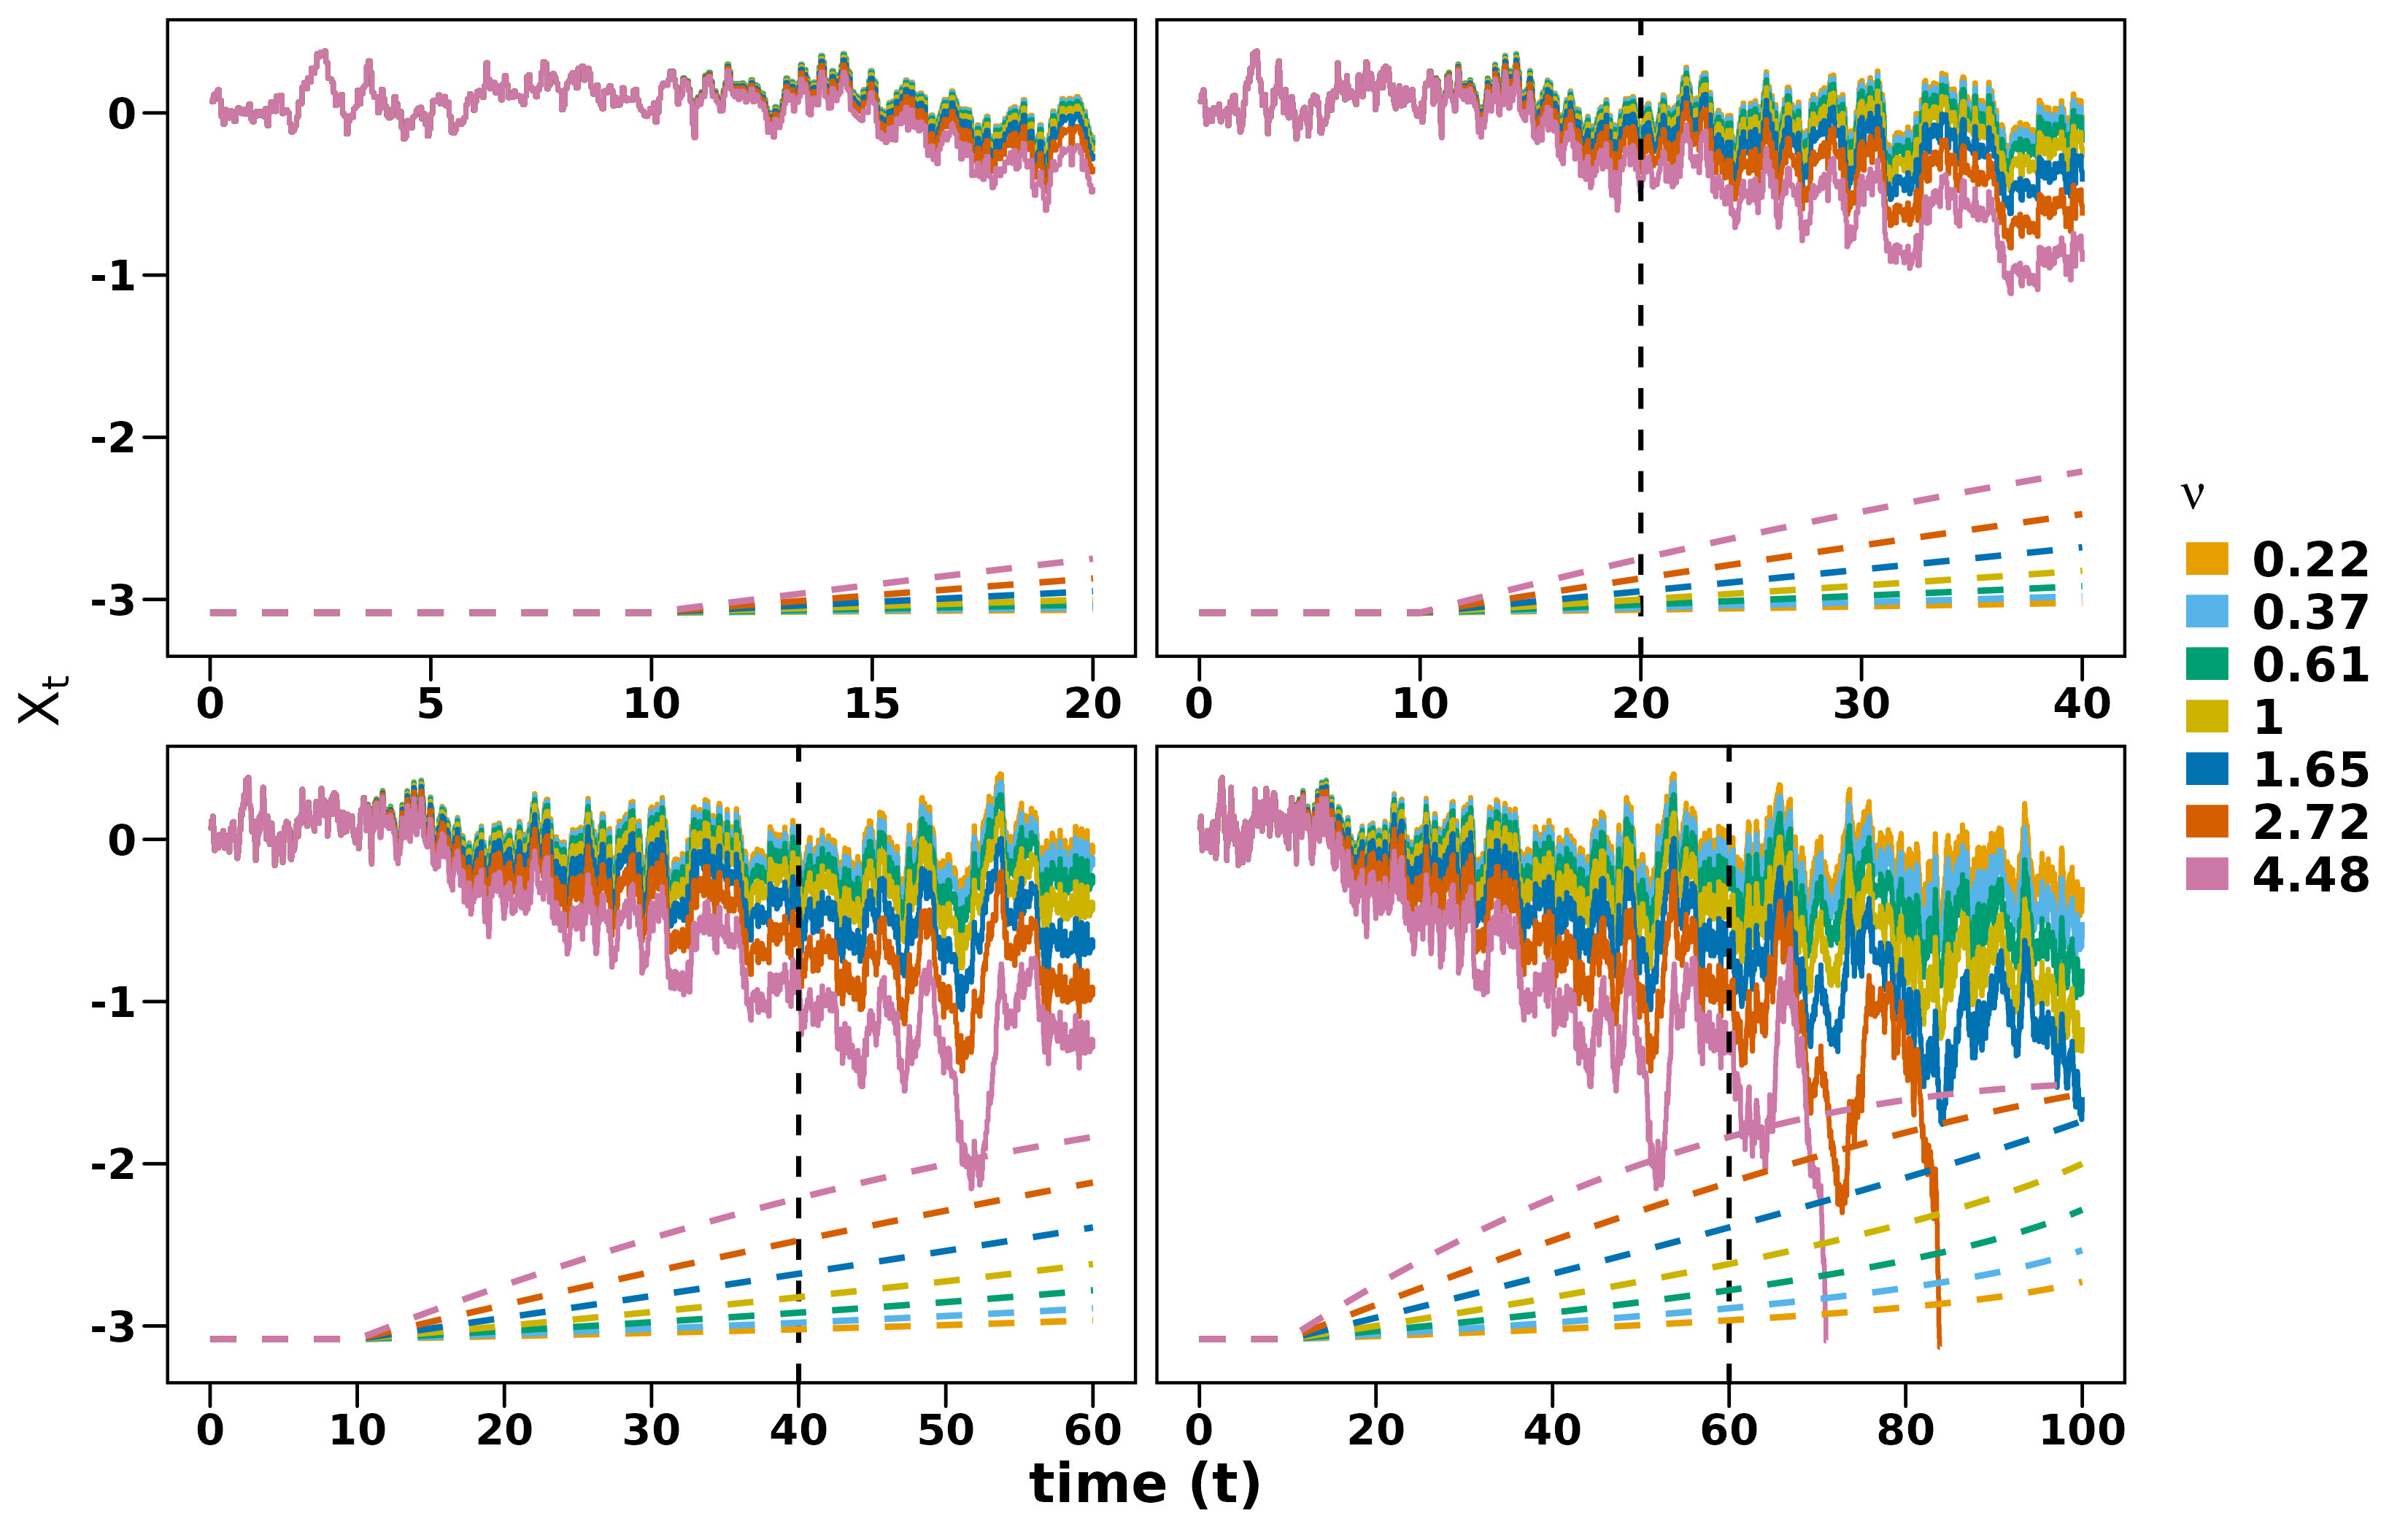
\includegraphics[scale = .13]{figures/mu_simulations_discussion_plot.jpeg}
    \caption{Sample paths for varying $\nu$ with the same realizations from the brownian motion cut at different points in time.}
    \label{figure:mu_simulations_discussion_plot}
    \end{center}
\end{figure}\\
This example is of course constructed for the sake of illustration and the following points might not always hold. However, Figure \ref{figure:mu_simulations_discussion_plot} is a clear example of some of the difficulties that can arise with regard to the estimation of the $\nu$-parameter. In each facet, the vertical dashed line marks the point in time up to which the facet before it ran. The colored dotted lines in the plots are the unstable fixed points that if crossed before the tipping point most likely result in the process experiencing noise-induced tipping. When this happens we can no longer predict a bifurcation tipping. Furthermore, due to noise-tipping the process is no longer close to the stable fixed point, whence there is no information about $\nu$ in the samples.

Conversely, we still need to have quite a long series of observations within the dynamic part of the process to be able to distinguish between the paths. We are only 240 observations within the dynamic part in the upper left facet in Figure \ref{figure:mu_simulations_discussion_plot}, and we can barely tell the sample paths coming from very different values of $\nu$ apart. That is at least visually. However, as our experiments have shown estimating values even moderately far away from $\nu = 1$ results in difficulties for the optimizer. 

All in all, we might need more sophisticated optimization methods than \code{optim} to have success with estimating $\nu$. This could be achieved as we have already discussed, while another option is using automatic differentiation lately made more easily applicable in \code{R} via the \code{torch} framework \cite{torch}, or even hand coding the optimizers.

Another option is to develop the numerical optimizer even further, albeit its possibilities of finding fixed points for a range of values $t$ as required in the dynamical part are quite limited without some a priori given assumptions about the evolution of these fixed points. The strategy that might be applicable here is to provide the specific form of $\lambda$ used throughout and use it to create a sub-optimization problem. Though, we do not observe $\lambda$ directly, the sample paths should be close to the fixed point on average; assuming that the process does not tip due to noise, of course. With this, we could perhaps use non-linear least squares to regress $\mu_t$ on the samples. We did experiment a bit with this with the method \code{stats::nls} but only got limited success. Solving the non-linear least squares at every iteration of the optimization is rather computationally expensive and it was quite error-prone: At some iterations, the \code{stats::nls} failed due to other parameters such as $A$ making the problem infeasible. To avoid this we could for instance adopt the penalization of $A$ used in \cite{Ditlevsen2023}.\\\\
Another thing we tried was making the numerical Strang method purely numerical. That is, it should be implemented such that the user merely provides the data, the specific model one wants to fit and the usual values required for optimization. In other words, the user should not need to provide the Lamperti SDE nor even the Lamperti transform (\ref{eq:lampertiDefinition}) here. The only additional thing the optimizers needs is the diffusion coefficient of one's model, i.e. ones choice of model. To achieve an estimator from this the method must construct the Lmaperti transform etc. numerically and then do the same steps as the other numerical Strang method does. We actually managed to implement a prototype of this. Yet, the computational speed of the method became the bottleneck of development; it took too long to evaluate the likelihood even once for the method to ever be viable. Now, a popular raison d'être of numerical methods could be that they allow us to use complex estimators without going through extensive calculations. And while simplifying the calculations necessary down to nothing whatsoever would be ideal, the method as is still provides a significant reduction in number of manual computations needed. Furthermore, it is uncertain if we would be able to match the results shown in Figure \ref{figure:ARE_dist_linear_noise} or \ref{figure:ARE_dist_numeric_F_diffusion}, if we automated the calculations further. In addition, it is to be expected that a user wanting to apply these methods would be able to find the Lamperti transform and compute the Lamperti SDE with Itō's formula, which is all the numerical Strang based method requires. This further cements keeping the numerical Strang method as it is.\\\\
We already touched on the idea of using the Strang splitting scheme to construct a score function. Now, a third way to use this scheme could be to construct martingale estimation equations for stochastic differential equations that are more complicated than the Pearson diffusions, e.g. the dynamic part of the process. As with our idea of using Kessler's method on the stochastic differential equation in the splitting, this method does not use the Lamperti transform of the process. To see this more easily, consider the square root-based dynamical part of the saddle-node normal form model
\begin{align}
    \mathrm{d}X_t = -(A(X_t - m)^2 + \lambda_t)\mathrm{d}t + \sigma\sqrt{X_t}\mathrm{d}W_t \label{eq:squareSplittingDiscussion}
\end{align}  
The following splitting can also be found in section \ref{subsubsec:squarerootDynamic}
\begin{align}
    \mathrm{d}X_t^{[1]} &= -\alpha(\lambda)\left(X_t^{[1]} - \mu(\lambda)\right)  \mathrm{d}t + \sigma \sqrt{X_t^{[1]}} \mathrm{d}W_t, \label{eq:squareRootSplit1_discussion} \\
    \mathrm{d}X_t^{[2]} &= - A \left(X_t^{[2]} - \mu(\lambda)\right)^2 \mathrm{d}t, \label{eq:squareRootSplit2_discussion}
\end{align}
with $\alpha(\lambda) = 2\sqrt{-A\lambda_t}$ and $\mu(\lambda) = m + \sqrt{-\frac{\lambda_t}{A}}$. As we mention in that part of the appendix this is applying the splitting heuristic from \cite{SplittingSchemes} to (\ref{eq:squareSplittingDiscussion}). However, what this gives us is an SDE (\ref{eq:squareRootSplit1_discussion}), for which we can construct martingale estimation equations. For the Strang composition, we recall that based on Figure \ref{figure:StrangAndLieTrotterPlot} the flow is a non-linear transform of the solution to the SDE (\ref{eq:squareRootSplit1_discussion}). So constructing the estimation equations for the whole flow is a matter of using a result about the relationship between eigenfunctions, $p_n(x)$ and eigenvalues $\lambda_n$ for a process such as $X_t^{[1]}$ and transformations of that process with functions such as $\varphi_2$. It turns out \cite[remark on p. 41]{StatisticalMethodsForSDE} that in this case the eigenfunctions are $p_n\left(\varphi_2^{-1}(x)\right)$, whereas the eigenvalues remain the same. Still, it is unlikely that we would be able to get the conditional mean and variance of the flow from these eigenfunctions and eigenvalues, so in the remaining calculations one has to use a few more results from the theory of estimation equations than what has been presented here.
\newpage
\subsection{Tipping of the AMOC}
Taking Figure \ref{figure:surival_curve_taus} and Table \ref{table:tipping_quantiles} as our starting points of the discussion, it is clear that all the models indicate tipping to be \textit{more} than likely within the next 140 years. By "likely" we understand the 66\% confidence interval that is used by the Intergovernmental Panel on Climate Change \cite{Ditlevsen2023} and across all models and fingerprints there is at least an $83.5\%$ chance of tipping occurring before the end of the year $2169$. What specific range of years the tipping of the AMOC is likely within varies a bit according to the different models. Still, all the \textit{estimates} from the data lie within medio 21st century and primo 22nd century signifying some form of overall agreement.\\\\
We did not investigate penalization on the models, but it would be interesting to implement some sort of penalization on $A$ into the $t$-diffusion-based model as well. To get an idea of how this could affect the estimates of the tipping time consider pairs of estimates of tipping year and $A$ stratified after model
\begin{figure}[h!]
    \begin{center}
    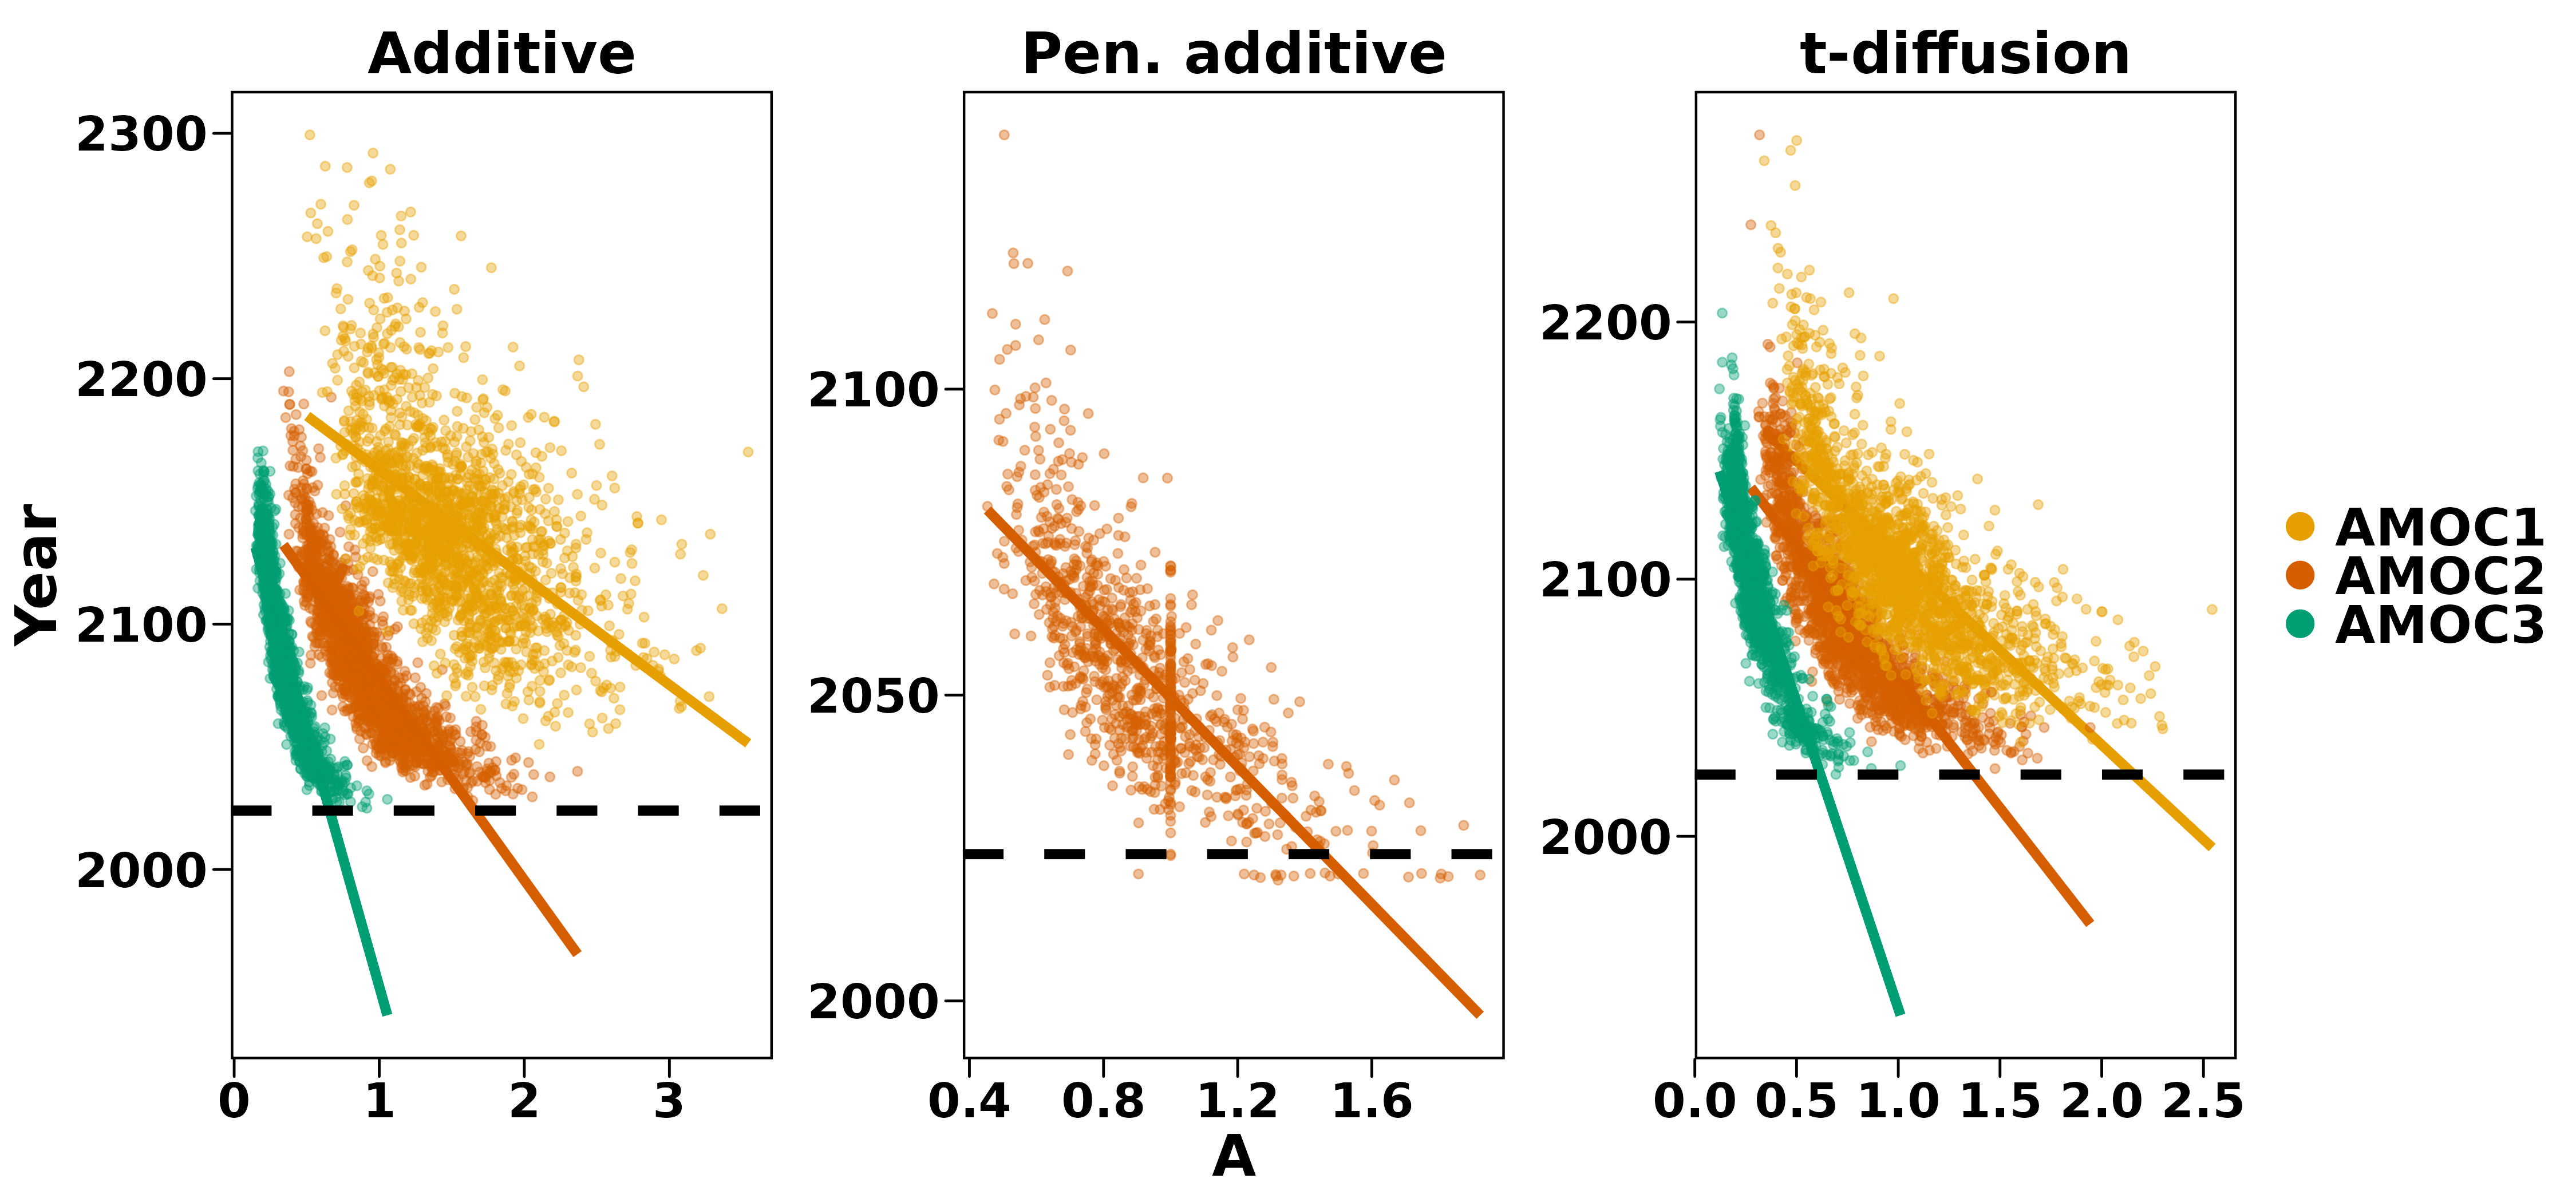
\includegraphics[scale = .082]{figures/correlation_between_A_and_tau_plot.jpeg}
    \caption{Pairs of estimates of tipping year and $A$ grouped by model and fingerprint}
    \label{figure:correlation_A_and_tau}
\end{center}
\end{figure}\\
The straight lines in the graphs are linear normal models fitted to the stratified samples they share color and facet with. In all cases, there is a strong negative correlation between the estimate of $A$ and -the tipping year; small values of $A$ tend to be have tipping estimates far in the future and vice versa. Indicating that if we want to avoid heavy-tailed estimators of $\tau_c$ we might want to penalize values of $A$ below 1 as done in the paper.

However, as seen in the graph in Figure \ref{figure:correlation_A_and_tau} this creates a clear bias towards $A = 1$. Actually, one could argue that the penalizations might have hurt the optimization somewhat. Note the clear cluster of points forming around $A = 1$ in the middle graph of Figure \ref{figure:correlation_A_and_tau}. This is likely a result of penalization of values below $A$ resulting in the optimization returning values \textit{really} close to $A = 1$. In fact, a closer investigation reveals that penalization results in $12.4\%$ of estimates of $A$ being closer than $0.0005$ units away from $1$, whereas the proportion of estimates of $A$ with an absolute distance of just $0.000025$ to $1$ is still $7.9\%$. While we of course expect the distribution to shift towards $1$ for values that would have been much smaller than $A = 1$, so many values this close to $1$ is a bit concerning and could indicate that there is something wrong with the optimization or penalization. 

Yet, looking at the source code nothing particular from the objective function has stood out in this regard. In the optimization itself, one thing to note is that the initial value of $A$ is 1, as in our application. There is a chance that the many estimates around the value 1 are caused by the optimization not being explorative enough. As mentioned, the paper uses the \code{Nelder-Mead} algorithm for optimization. This algorithm is generally considered more exploitative than explorative. While this exploitive nature ensures we do not get the extreme estimates that our methods sometimes suffer from, there is the risk of getting stuck in local minima. To see if this is the case here, we implement a tracer into the objective function. This allows us to retrieve the parameters and objectives at every iteration and potentially diagnose any problems. We sketch the trace of each of the parameters, where we have used the penalized additive model on the AMOC2 fingerprint with starting values $A = 1$ and $\tau_c = 100$. 
\begin{figure}[h!]
\begin{center}
    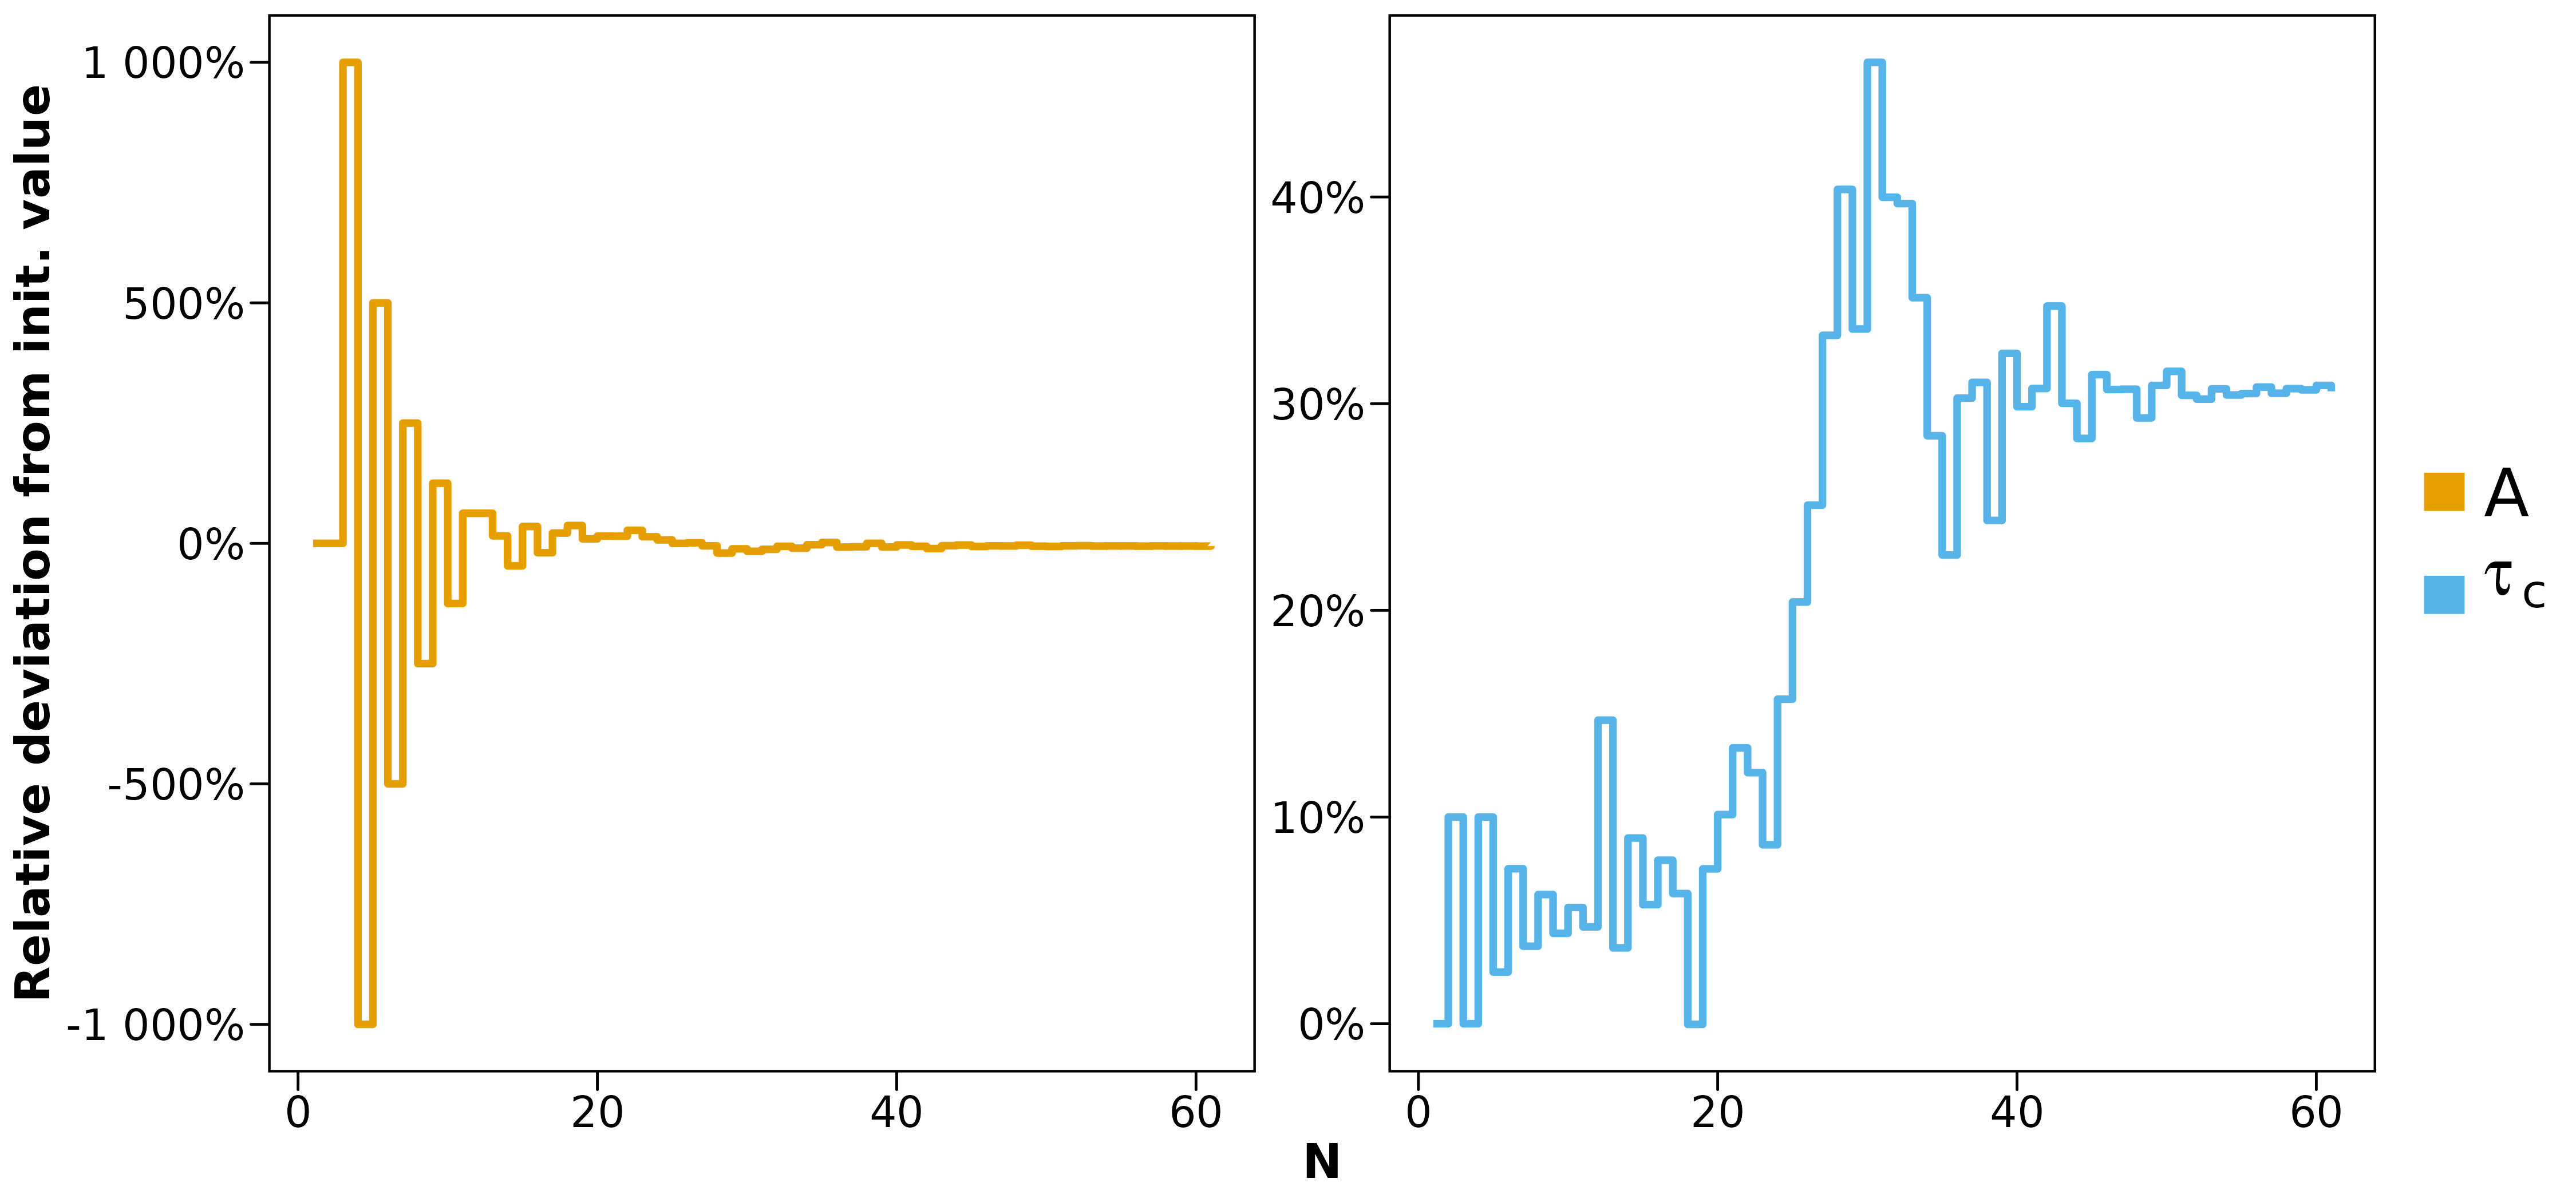
\includegraphics[scale = .075]{figures/trace_plot.jpeg}
    \caption{Trace plot of parameter values at each step of the optimization showing the relative deviation from the initial values $A = 1$ and $\tau_c = 100$.}
    \label{figure:trace_plot}
\end{center}
\end{figure}\\
However, in this example there is no lack of exploration of the $A$-parameter; the optimizer searches among parameter values far away from the starting value. The same thing can be said about $\tau_c$ though its trace appears more guided overall. Of course, this is only one trace and we would need to examine more traces to reject this potential problem more confidently. On the other hand, the underlying cause might just be the fact that the penalty is applied at a discrete level $A<1$; this could potentially push values of $A$ moderately close to 1 closer, such that many estimates would be quite close in this way.

Regardless of whether it is caused by something undesired, having many values of $A$ around $1$ limits the range of values of the tipping, shifting $\tau_c$ in the specific direction as argued by the negative correlation in Figure \ref{figure:correlation_A_and_tau}. Again, there is nothing inherently wrong with the correlation of the estimates, but it becomes an issue, if there is something problematic in the optimization phase such as the potential problem illustrated here. And although we have not been able to establish the exact underlying cause, there could be reasons to believe that something in the optimization should be changed. Whether that is the type of penalization, the penalization altogether or something completely different, we do not answer here.

Apart from this, we also discovered a minor bug in the implementation of the objective function for the dynamic part of the additive model that is in the supplementary material of the paper. The bug has since been corrected and although the estimates are a bit different, it has been checked that the distribution of the tipping time stays roughly the same after the correction. This means the arguments and comparisons made with results from the paper still hold. For this reason, we do not redo all the computations to recreate the distributions of \cite{Ditlevsen2023}. To this end, it is worth mentioning that there are other minor differences in the choices made between the estimation methods of the paper and this project such as whether $\sigma$ or $\sigma^2$ is estimated, what optimization algorithm is used, where $A$ is allowed to be negative etc.
These differences can compound making the results quite different overall. 

With this in mind, we get $2054$ for the tipping time with the exact penalization used in the paper applied in our objective function for the additive model. This is rather close to the original result, confer Table \ref{table:tipping_quantiles}, which further justifies the use of the results from the paper in spite of the minor discrepancies. Again, the result we just presented comes with the caveat that the implementation from the paper might not agree completely and it might have been a bit naïve of us to select the exact same penalization value for the optimization and not determine it via cross-validation for instance. However, it is done in the way to try and ensure some overall comparability to the original implementation.\\\\
Returning to the selection between the two models; in our initial discussion (below Figure \ref{figure:OU_t_diffusion_QQ_plot}) we favored the $t$-diffusion model as its uniform residuals resembled that of the standard Gaussian better overall — suggesting a better fit. Confer Table \ref{table:tipping_quantiles} the models agree on the estimated tipping times and their confidence intervals — for the most part. On the AMOC2 data, they are almost in complete agreement. Interestingly, the additive model generally puts tipping later on the AMOC1 fingerprint and earlier on the AMOC3 in comparison with the $t$-diffusion-based model. A strength in the $t$-diffusion model here is that it is more robust against the choice of fingerprint than the additive model; this can also be seen by how close the survival curves in Figure \ref{figure:surival_curve_taus} are.

Generally, we have argued for the $t$-diffusion model. It seems to provide a better fit overall, while also ensuring robustness without the need to tune hyperparameters for penalization. However, with the limited tools we have to differentiate between the models, one could argue that the real significance of using multiple different stochastic terms with the same deterministic drift, as we have with the construction \ref{eq:standardStochasticForm}, is that it adds a different layer to the robustness analysis. If one can illustrate an effect in the deterministic part of a stochastic differential equation using several models with different diffusion terms, then it would strengthen our belief in that estimate as it is clearly less dependent on the model one uses. We succeeded in doing so with two models, though, preferably we would like to be able to apply other models as well, but of the models we have shown here only two are applicable to negative observations. There might be ways to adapt the diffusion terms in the other models to extend them to reals, while still keeping their structure. Another solution could be to use some monotone map from the reals onto the positive real numbers, e.g. the exponential function. As our domain knowledge on climate physics is somewhat limited, we refrain from doing so here.\\\\
A completely different option is instead of letting the ramping of the bifurcation parameter, $\lambda_t$ depend on time in a way that bifurcation inevitably occurs, we could model the bifurcation parameter using, say, a linear normal model. This allows us to use covariates e.g. the $\mathrm{CO}_2$ levels in the atmosphere. A specific model that we have thought about is the following
\begin{align}
    \lambda_x= \beta_2 x + \beta_1, \label{eq:alternativeLambda}
\end{align}
where $x$ is the global mean $\mathrm{log}$-$\mathrm{CO}_2$ in the atmosphere. The objective here would be to estimate $\beta_1$ and $\beta_2$ and we would find the critical value by solving $\lambda_x = 0$ for $x$, i.e. $\hat{\lambda_c} = -\frac{\hat{\beta_1}}{\hat{\beta_2}}$; giving us the $\mathrm{CO}_2$ level at which tipping occurs instead of the point in time. A minor point to note here is that $\hat{\lambda_c}$ is not a very well-behaved estimator. Being the ratio of two Gaussian variables it has for instance no mean. Other variations of a model with covariates could be an extension of the linear regression ramping model, where we introduce a parameter like $\nu$ in an exponent analogously to (\ref{eq:lambdaRampDefinition}), turning the sub-problem into a non-linear regression problem. \\\\
Nevertheless, this model would not only be different to estimate in, it would somewhat shift our perspective on the tipping model. In the \textit{time to tipping} type models there are of course the built-in assumption in the ramping (\ref{eq:lambdaRampDefinition}) that the development in the past continues going forward and the tipping time should of course be taken with this caveat. Though, what exactly drives the evolution of $\lambda_t$ is difficult to reason about, so it is hard for us to intuitively see if the evolution in the future follows the expected path or deviates. On the other hand, a tipping $\mathrm{CO}_2$ value could be easier to communicate and we can easily measure if the concentration of $\mathrm{CO}_2$ in the atmosphere is below the threshold. 

Furthermore, the two models invite us to think in completely different ways in the first place: That ramping does not necessarily continue can be hard to remember for a layperson; in that light, a tipping time type model seems like a crystal ball predicting an inevitable event in the future. On the other hand, with the \textit{tipping level} type model, it is easy to fall into the trap of seeing tipping as a phenomenon that necessarily occurs at specific $\mathrm{CO}_2$ levels. That is assuming a form of causality, the model does not let us reason about. However, the tipping level type excels in encouraging us to think about the system in a structured manner. One could for instance ask questions about what levels of $\mathrm{CO}_2$ we should avoid for it to be "likely" that the system does not reach a tipping point. \\\\
Finally, if we had both types of models they could, and arguably should, be used in conjunction. With them, we could check if the time of tipping aligns well with our current $\mathrm{CO}_2$ projections. That is, does the projected time for our reaching the critical $\mathrm{CO}_2$ level agree with the critical time in the tipping time type models? In the positive case, this would be an excellent tool to make the estimates even more convincing, whereas the other case lets us ask interesting questions as to why this could be the case.

\subsection{Conclusion}
In sum, we have proposed two types of natural extensions to the stochastic normal form of the saddle-node bifurcation. Simulation studies where we put realistic limitations on the knowledge of the initial parameters have shown that we so far can estimate the parameters of all six variations fairly well as long as we omit the $\nu$-parameter. It was somewhat unsatisfactory that we could not get the estimation of the $\nu$-parameter to work in cases, where we initialized the parameter in $1$; corresponding to assuming the simpler ramping model from previous work. However, we did reflect on alleys to go down which could lead to a more numerically stable method for the estimation of $\nu$.\\\\
At the same time, we managed to contribute with new insights into the potential tipping point in the climate system the AMOC. Using the additive model without penalization and a model based on the diffusion term from the $t$-diffusion to estimate the tipping point of this system. We found results that find themselves in the same range as what was found in the original work on the subject. As we showed, we do, however, have slightly more conservative estimates — putting tipping to be likely within the next 140 years across all models and fingerprints. In general, we saw a much heavier tail than the original estimates of the year of tipping. However, for most models and fingerprints we saw it was likely within the next 100 years, which aligns well with the previous work. Finally, we mentioned interesting paths that future research may take and proposed and reflected on the general ease of interpretability of these models. 